\documentclass[a4paper]{article}

\usepackage[T1]{fontenc}
\usepackage[italian]{babel}
\usepackage[latin1]{inputenc}
\usepackage{graphicx}
\usepackage{float}
\usepackage[margin=2 cm]{geometry}
\usepackage{multirow}
\usepackage{multicol}
\usepackage{textcomp}
\usepackage{caption}
\usepackage{units}
\usepackage{amsmath}
\usepackage{mathtools}
\author{Alberto Bordin, Giulio Cappelli}
\title{Fibre ottiche}
\date{20-24 Novembre 2017}
\newcommand{\minitab}[2][l]{\begin{tabular}#1 #2\end{tabular}}


\begin{document}
	\maketitle
	
	\begin{abstract}
		 
	\end{abstract}

\section{To do}
\begin{itemize}
	\item scegliere errori attenuazione
	\item verificare valori $L$ attenuazione
	\item fit con errori asimmetrici per l'attenuazione?
	\item sintetizzare supercazzola sugli errori dell'attenuazione
	\item errore su b nell'attenuazione
	\item discutere livello scrambler
\end{itemize}
\section{Teoria}

\section{Apparato sperimentale}

\section{Apertura numerica}

\subsection{Teoria}

\subsection{Presa dati}

2 tabelle

\subsection{Analisi dati}

2 plot con interpolazione quadratica o al massimo cubica

\newpage
\section{Attenuazione}

\begin{multicols}{2}

\subsection{Teoria}
In una fibra ottica si ha dissipazione dovuta allo scattering Rayleigh con le impurit� della fibra. La potenza dissipata � proporzionale a $\lambda^{-4}$, scopo dell'esperienza � verificare questa legge di potenza.\\
L'attenuazione $\alpha$, che � proporzionale alla potenza dissipata, � definita come 
\[\alpha = \frac{10}{L} \log \left | \frac{ P_{in}}{P_{out}} \right | \quad\textrm{     [dB/km]}\]
dove $P_{in}$ e $P_{out}$ sono, rispettivamente, la potenza in ingresso e la potenza in uscita ad un tratto di fibra di lunghezza $L$.

\subsection{Apparato sperimentale}

\begin{figure}[H]
	\centering
	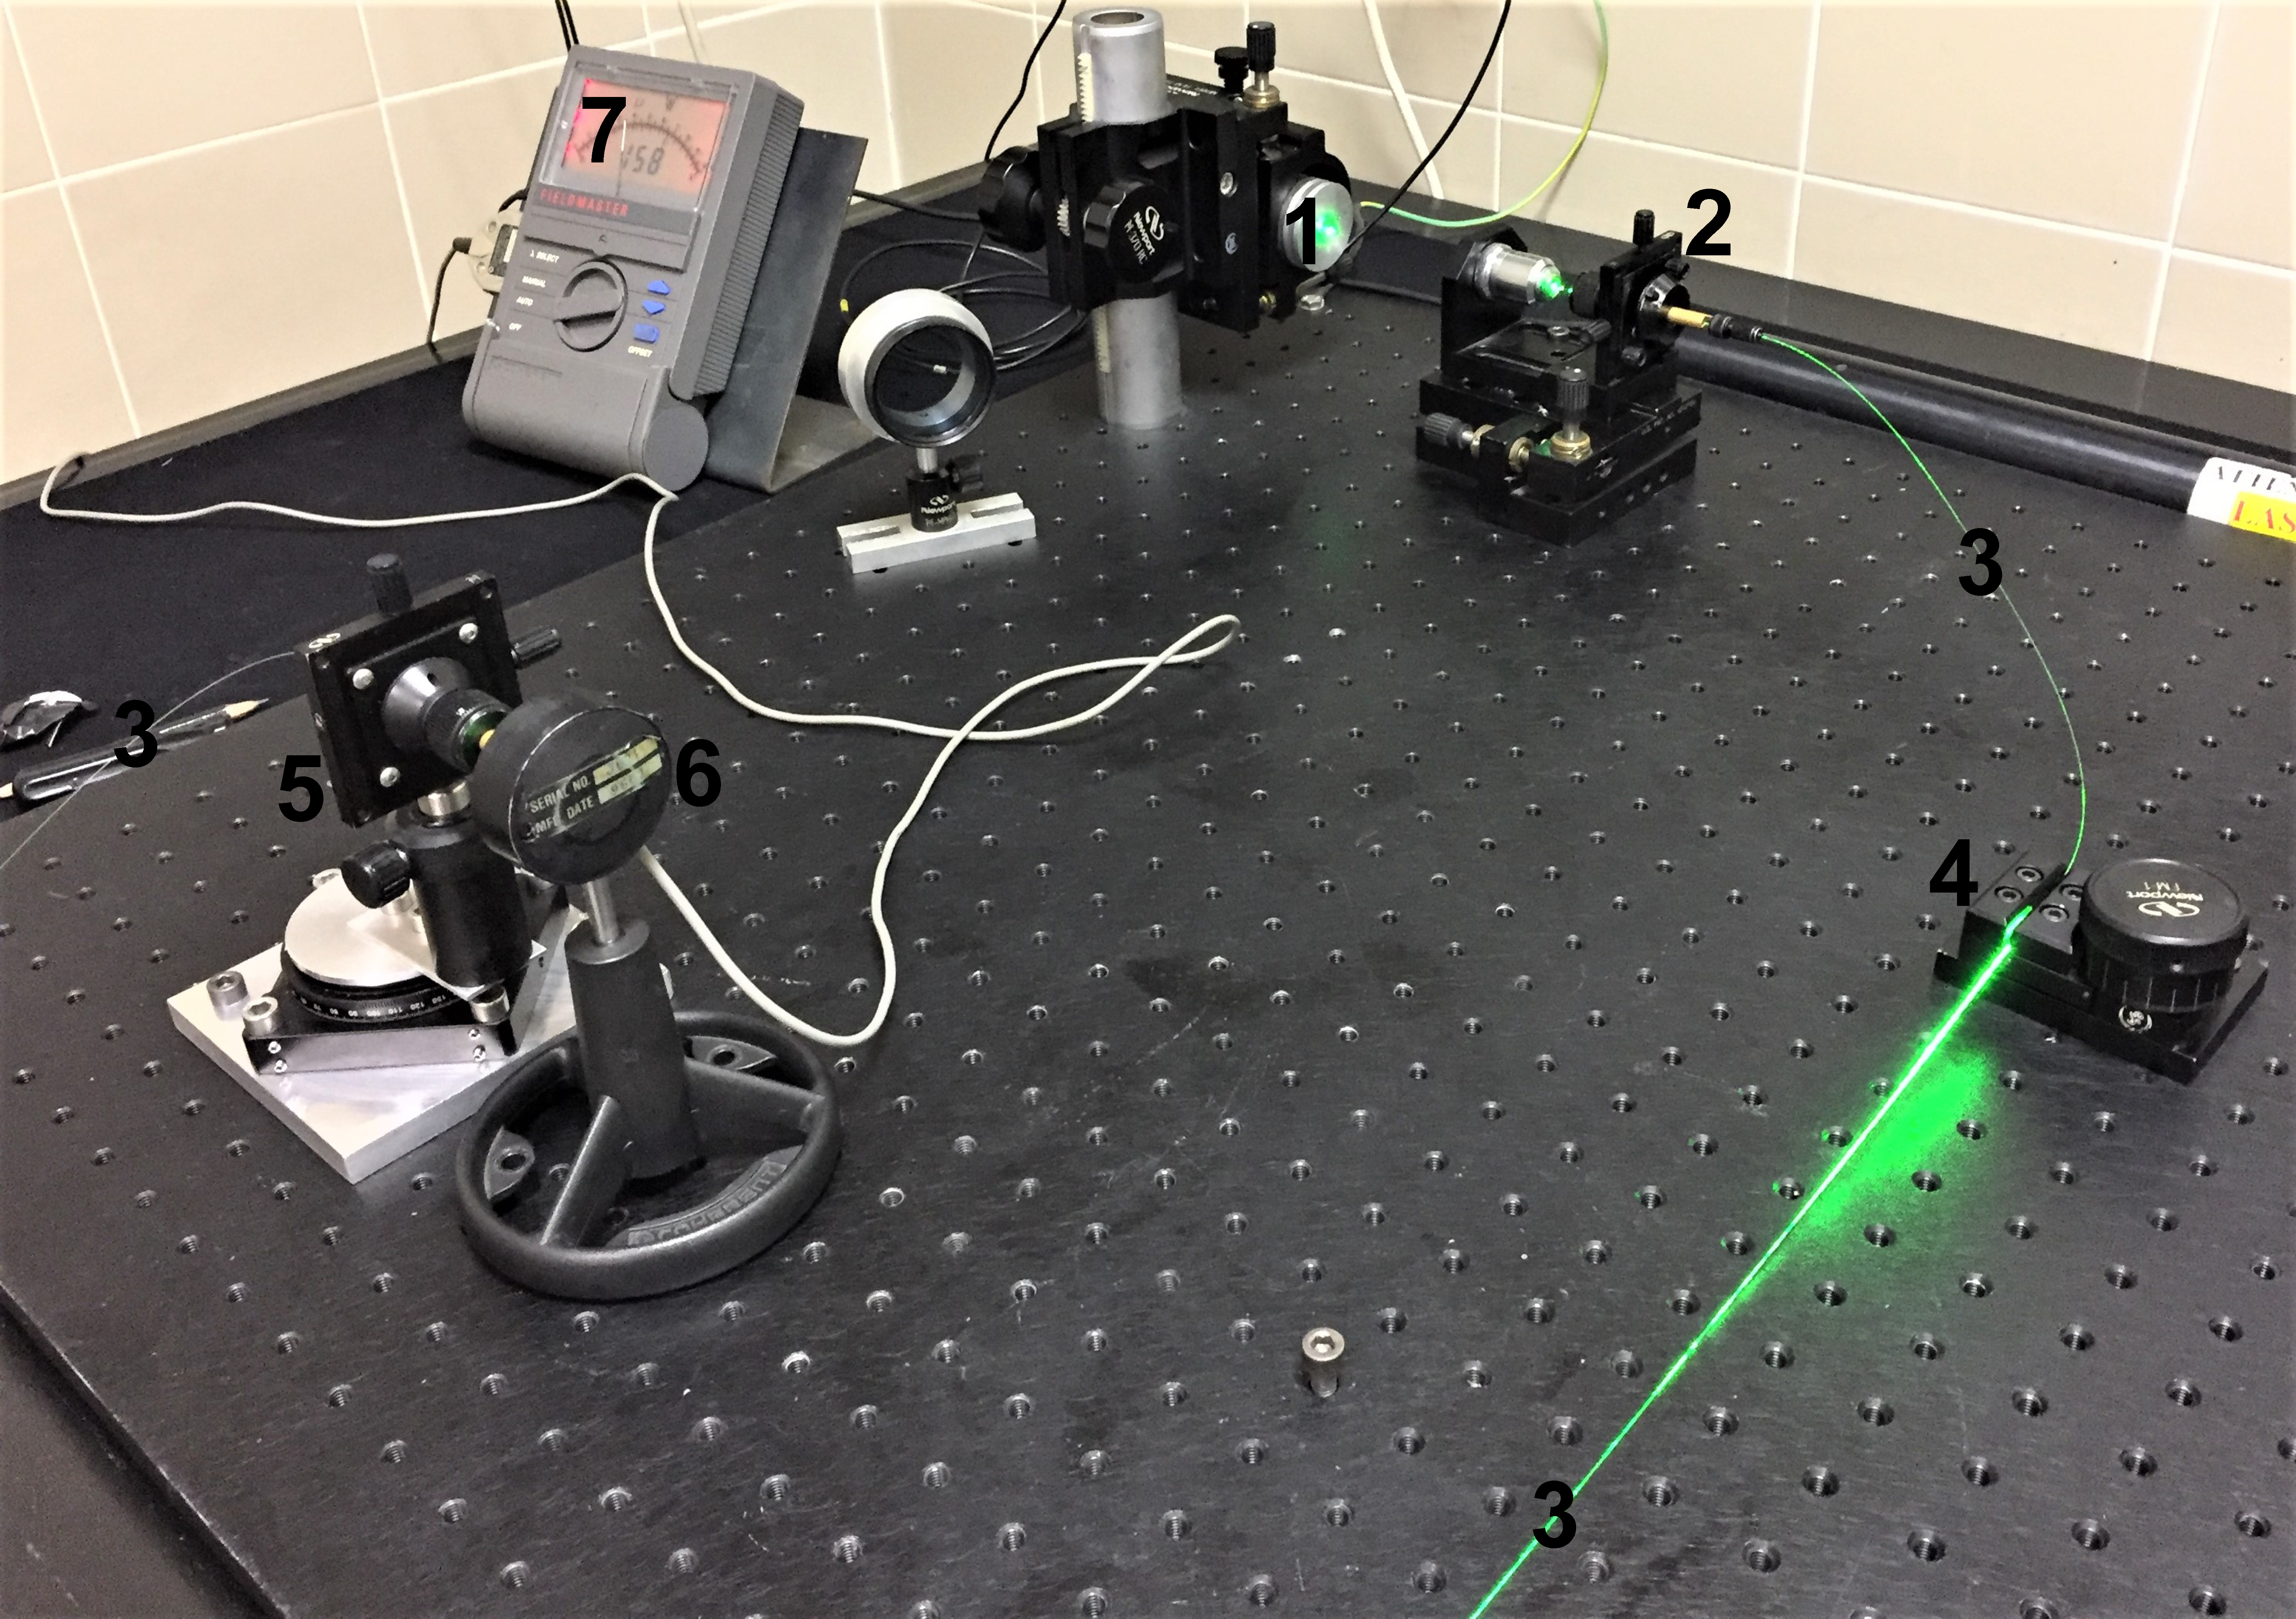
\includegraphics[width=0.5\textwidth]{apparato_attenuazione.pdf}
	\caption{Apparato sperimentale per la misura di attenuazione.}
	\begin{enumerate}
		\item Laser
		\item Lanciatore (con obiettivo 20x)
		\item Fibra ottica multimodo F-MLD
		\item \textit{Scrambler}: una sorta di piccola morsa ondulata che serve ad eliminare i modi spuri.
		\item Uscita della fibra
		\item Sensore del \textit{power meter}
		\item Schermo del \textit{power meter}
		\item Rotolo da $\sim300$ m di fibra ottica
	\end{enumerate}
	\label{fig:apparato_attenuazione}
	\begin{minipage}{0.23\textwidth}
		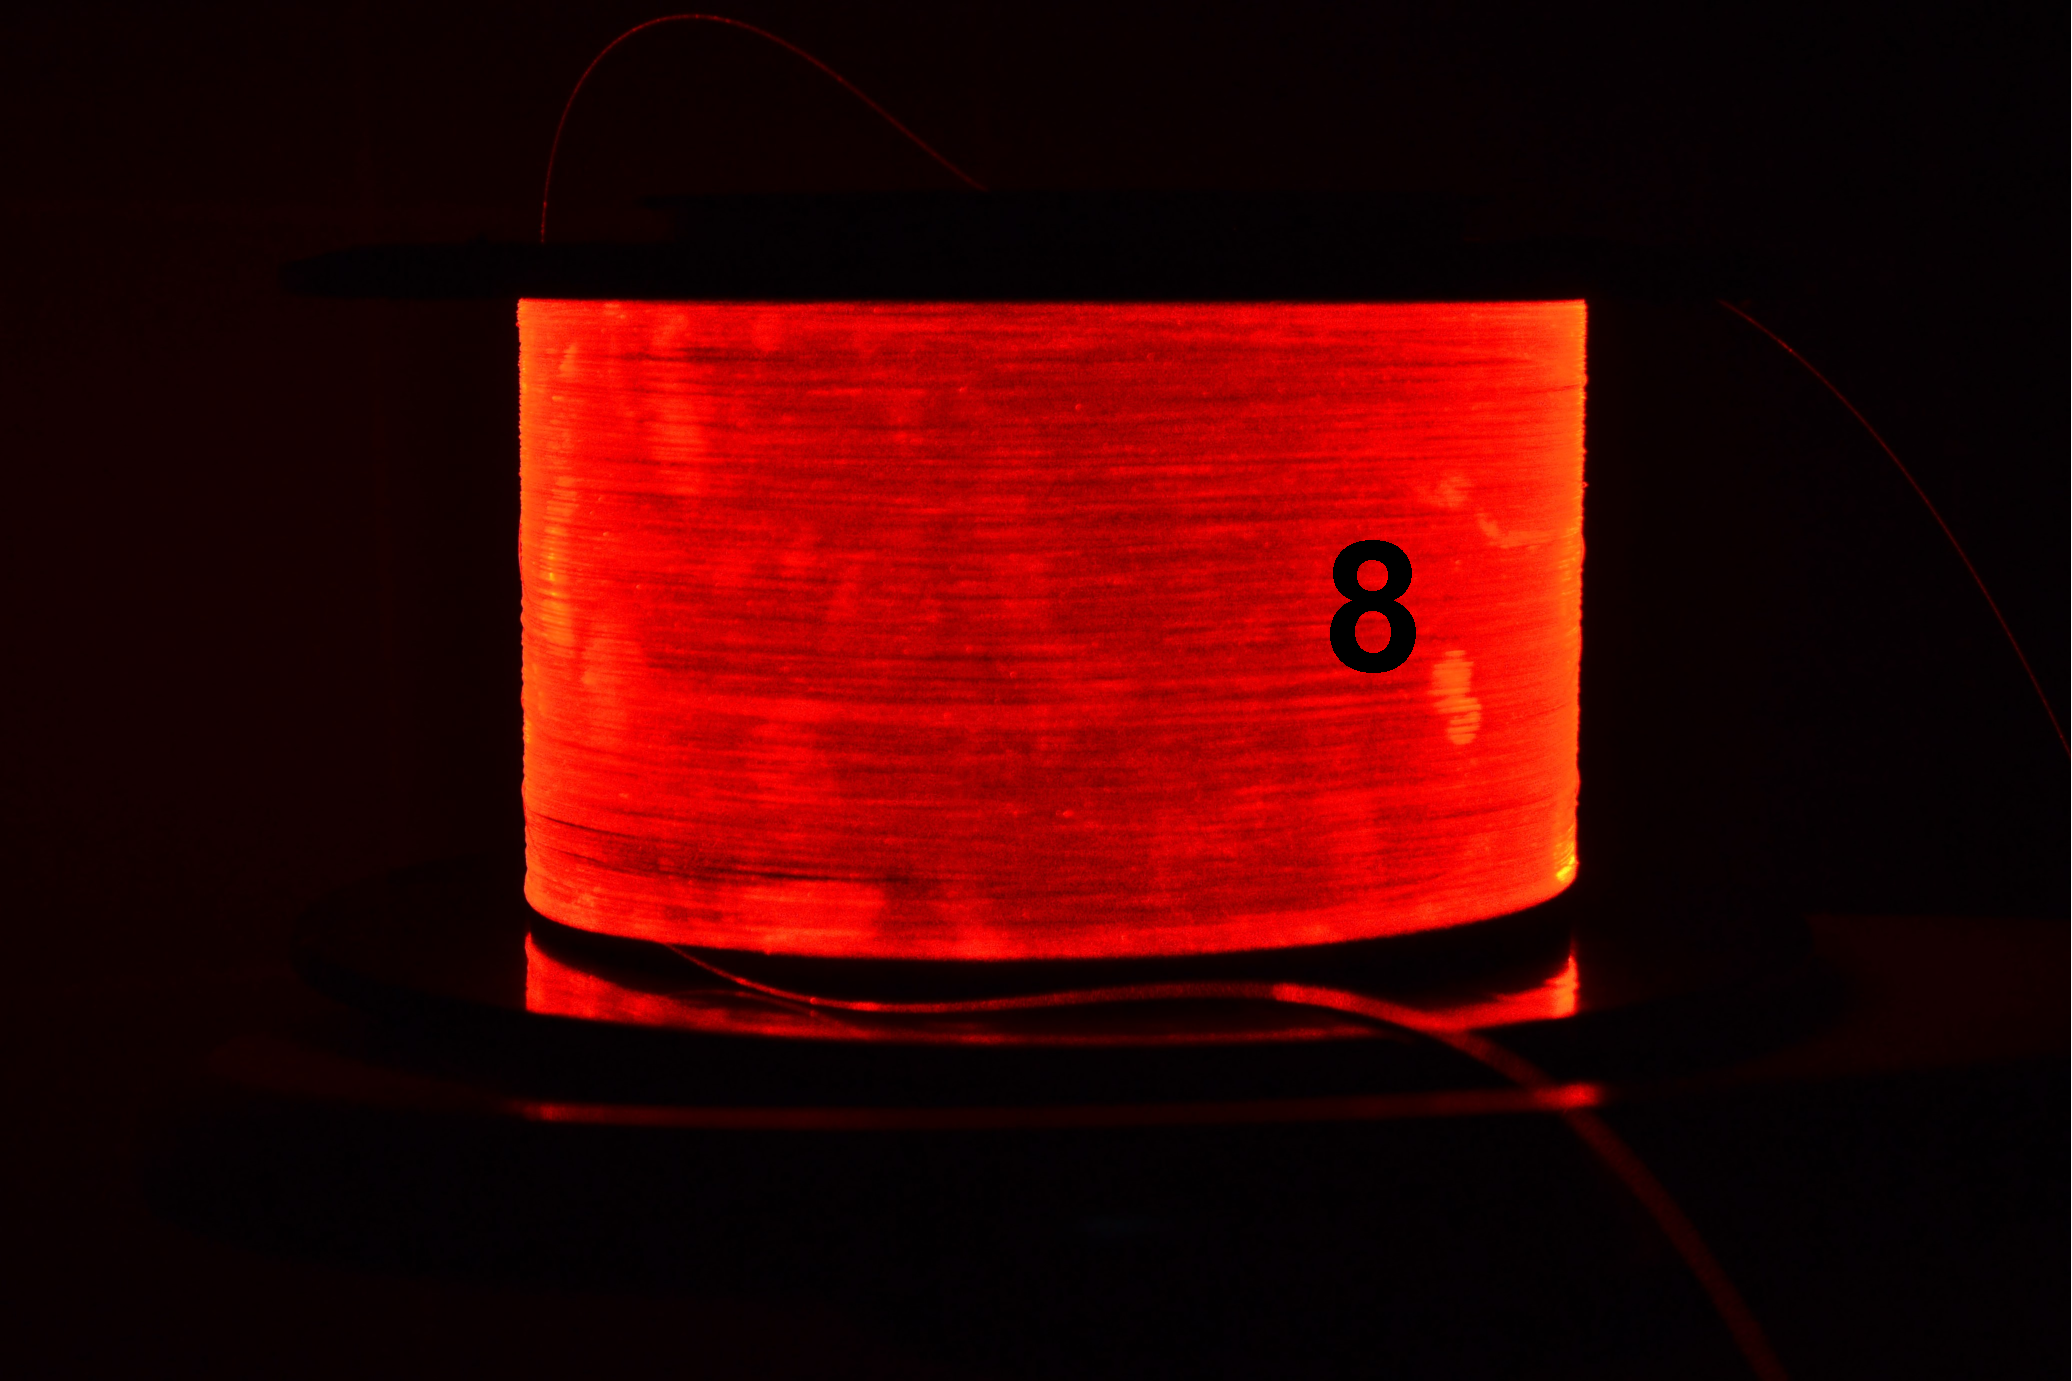
\includegraphics[width=\textwidth]{bobina_rossa.pdf}
	\end{minipage}
\begin{minipage}{0.24\textwidth}
	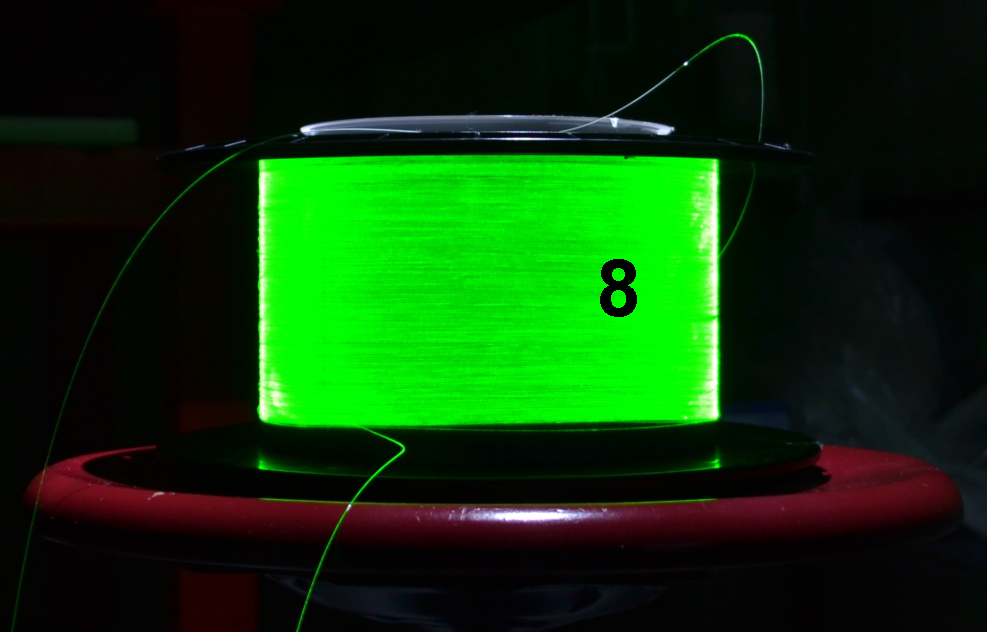
\includegraphics[width=\textwidth]{bobina_verde.pdf}
\end{minipage}
\end{figure}

\subsection{Presa dati}
La misura � svolta in due passaggi.
\begin{enumerate}
	\item Si lancia in fibra un fascio laser e si misura la potenza in uscita: $P_{out}$.
	\item Si taglia la fibra a 2 metri dal lanciatore e si misura di nuovo la potenza in uscita: $P_{in}$.
\end{enumerate}
Quindi $L$ � la lunghezza del rotolo meno i 2 m tagliati.

In Tabella \ref{tab:alpha} riportiamo le potenze misurate.
\begin{table}[H]
	\centering
	\begin{tabular}{|c|cccc|}
		\hline
		$\lambda$ [nm] & $L$ [m]  & $P_{out}$ [mW]& $P_{in}$ [mW]& $\alpha$ [dB/km] \\
		\hline
		633  & 293.5(5) & 0.598(18) & 1.63(5) & 14.8(6)\\
		
		532 & 291.3(5) & 0.156(5) & 1.47(4) & 33.4(6)\\
		\hline
		\hline
		633  & 289.2(5) & 0.83(2) & 2.44(7) & 16.2(6)\\
		
		532 & 287.1(5) & 0.320(10) & 2.80(8) & 32.8(6)\\
		\hline
	\end{tabular}
	\caption{Misure di $P_{in}$ e $P_{out}$ e calcolo dell'attenuazione.}
	\label{tab:alpha}
\end{table}
Come si nota in Tabella \ref{tab:alpha} per ogni laser abbiamo fatto 2 misure di $\alpha$. Infatti gli $\alpha$ ricavati alla prima presa dati (prime 2 righe della Tabella \ref{tab:alpha}) risultano incompatibili, a detta del professore, con quanto misurato dai nostri colleghi predecessori. Quindi a fine settimana, sotto la testimonianza oculare del tecnico di laboratorio, abbiamo ripetuto le misure di attenuazione (ultime 2 righe di Tabella \ref{tab:alpha}) ritrovando dei valori simili a quelli misurati ad inizio settimana. Pertanto non riusciamo a spiegare la discrepanza con quanto misurato negli anni passati.

\subsubsection*{Discussone degli errori}
Gli errori su $L$ sono relativamente piccoli (abbiamo scelto 0.5 m) perch� siamo appena il secondo gruppo che utilizza il rotolo di fibra. Ogni misura aggiunge un errore di $\sim5$ cm a causa dello spellamento della fibra, quindi gli ultimi gruppi avranno un errore di qualche metro.

In Tabella \ref{tab:alpha} l'errore sulla potenza � il 3\% indicato sul datasheet del \textit{power meter}, questa scelta � discutibile, quindi merita un approfondimento. Infatti nel datasheet il sudetto 3\% � indicato come errore sull'accuratezza, cio� errore di calibrazione. Tuttavia nel calcolo di $\alpha$ entra il rapporto di $P_{in}$ e $P_{out}$, pertanto l'errore di calibrazione, che � un errore sistematico, si cancella: conta solo l'errore statistico. Quindi in prima analisi avevamo scelto per $P$ gli errori di digitalizzazione (sommati a quello che sul datasheet � indicato come \textit{Power Noise Level} = 2 $\mu$W nel caso che quest'ultimo non fosse trascurabile). Ma tale scelta portava a degli errori su $\alpha$ di 0.02 dB, che rende le 2 misure dell'$\alpha$ relativo alla stessa $\lambda$ del tutto incompatibili.\\
Dato che eccezionalmente abbiamo due misure di $\alpha$, per ogni $\lambda$ possiamo stimare l'errore a posteriori con la deviazione standard sperimentale:
\begin{equation}
\begin{aligned}
\sigma_{(\lambda = 633)} = 0.9 \textrm{ dB/km}\\
\sigma_{(\lambda = 532)} = 0.5 \textrm{ dB/km}
\end{aligned}
\label{eq:sigma}
\end{equation}
Il valore di tale stima � simile a quello che si ottiene utilizzando il 3\% come errore sulle potenze (l'errore cos� ottenuto � 0.6 dB/km) ed � molto diverso dai 0.02 dB discussi sopra. La discrepanza potrebbe avere diverse origini e probabilmente viene da piccole e casuali alterazioni delle condizioni sperimentali, difficili da stimare. In ogni caso utilizzando il 3\% come errore sulle potenze l'errore su $\alpha$ viene sensato, quindi tanto vale lasciare quello, anche perch�
\begin{itemize}
	\item l'errore di calibrazione si cancella nel rapporto solo se $P_{in}$ e $P_{out}$ sono misurate nelle stesse identiche condizioni, che non � del tutto vero dato che tra una misura e l'altra cambia il fondo scala (da mW a $\mu$W), questo pu� comportare una differente calibrazione;
	\item gli errori di calibrazione indicati nei datasheet sono validi per qualche anno, e dato che i nostri strumenti sono preistorici non sappiamo veramente quale sia l'errore di calibrazione.
\end{itemize}
Nella Tabella 1 abbiamo lasciato gli errori di calibrazione del datasheet e la consegente propagazione, nell'analisi che segue abbiamo usato la deviazione standard dell'equazione \ref{eq:sigma}.
\subsection{Analisi dati}
Alle nostre misure si aggiungono i valori del datasheet della fibra, che riporta quanto segue:
\begin{table}[H]
	\centering
	\begin{tabular}{|c|c|}
		\hline
		$\lambda$ [nm] & $\alpha$ [dB/km] \\
		\hline
		850  & $\leq$ 4.0\\
		1300 & $\leq$ 1.5\\
		\hline
	\end{tabular}
	\caption{Attenuazione riportata nel datasheet.}
	\label{tab:alpha_n}
\end{table}
I valori di Tabella \ref{tab:alpha_n} sono problematici in quanto
\begin{enumerate}
	\item non riportano l'errore,
	\item indicano un $\leq$, che fa pensare ad un errore asimmetrico.
\end{enumerate}
Probabilmente il vero valore misurato dal rivenditore sar� stato di poco inferiore ai valori di Tabella \ref{tab:alpha_n}, ma non sappiamo di quanto n� con che errore.
Sperando che il rivenditore abbia riportato il corretto numero di cifre significative l'errore dovrebbe essere compreso tra 0.1 e 1 dB: in prima analisi scegliamo 0.1 dB.
Per i problemi appena discussi scegliamo, innanzitutto, di analizzare separatamente le nostre misure e i valori del datasheet (vedi Figura \ref{fig:attenuazione_coppie}).

\begin{figure}[H]
	\centering
	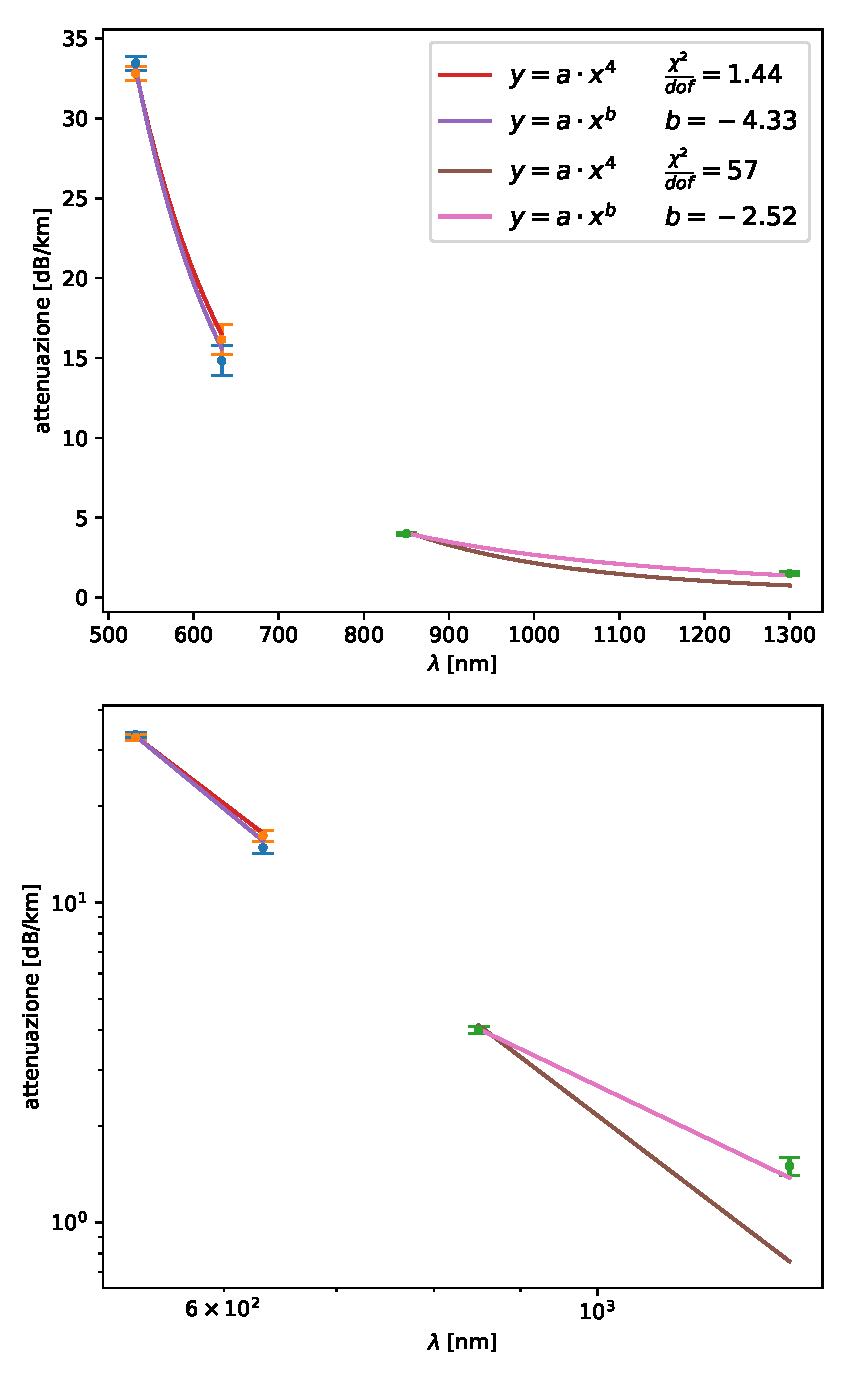
\includegraphics[width=0.5\textwidth]{attenuazione_coppie.pdf}
	\caption{Grafico dell'attenuazione in fibra ottica sia in scala lineare che bilogaritmica. In blu e arancione le nostre misure, in verde i valori del datasheet.}
	\label{fig:attenuazione_coppie}
\end{figure}

Per verificare la legge di potenza dello scattering Rayleigh secondo cui $\alpha \propto \lambda^{-4}$ eseguiamo 2 fit con funzioni di diverso tipo:
\begin{enumerate}
	\item $y = a \cdot x^4$ e guardiamo il $\chi^2$ per stabilire se il modello � valido,
	\item $y = a \cdot x^b$ e guardiamo se $b$ � compatibile con 4.
\end{enumerate}
Come si vede dalla legenda di Figura \ref{fig:attenuazione_coppie} le nostre misure non sono incompatibili con $\alpha \propto \lambda^{-4}$ mentre i valori del datasheet s�. In particolare dal grafico bilogaritmico si nota come i valori del datasheet non seguano la pendenza corrispondente a un $\lambda^{-4}$ (curva marrone in Figura \ref{fig:attenuazione_coppie}). Dobbiamo quindi concludere che o i valori riportati dal datasheet (per le problematiche sopra indicate) o gli errori da noi scelti sono incompatibili con il modello dello scattering Rayleigh. Non sappiamo se il problema sta negli errori o nelle carenze del modello, in ogni caso non riteniamo utile aggiungere altri parametri (come un offset) alla funzione di fit perch� non abbiamo abbastanza dati per eseguire un'appropriata analisi statistica.

Nonostante le incompatibilit� discusse sopra riportiamo per completezza gli stessi fit eseguiti per l'unione delle nostre misure e dei valori del datasheet. I risultati sono nella legenda di Figura \ref{fig:attenuazione_tutti}.

\subsection{Conclusioni}

Le nostre misure di attenuazione non sono incompatibili con il modello dello scattering Rayleig ($\alpha \propto \lambda^{-4}$), tuttavia abbiamo riscontrato le seguenti problematiche:
\begin{itemize}
	\item A detta del professore le nostre misure sono incompatibili con quanto misurato dai nostri predecessori. A scanso di equivoci abbiamo ripetuto le misure, ritrovando valori simili alla prima presa dati, quindi non sappiamo spiegare la discrepanza con le misure degli anni passati. L'unica differenza rispetto agli anni scorsi � il nuovo rotolo di fibra. Siamo curiosi di confrontare le nostre misure con quelle dei nostri colleghi di quest'anno.
	\item I dati riportati dal datasheet hanno molteplici problemi: non hanno un errore e sono riportati con un ambiguo $\leq$. Inoltre risultano incompatibili con $\alpha \propto \lambda^{-4}$.
\end{itemize}
	
\end{multicols}

\begin{figure}[H]
	\centering
	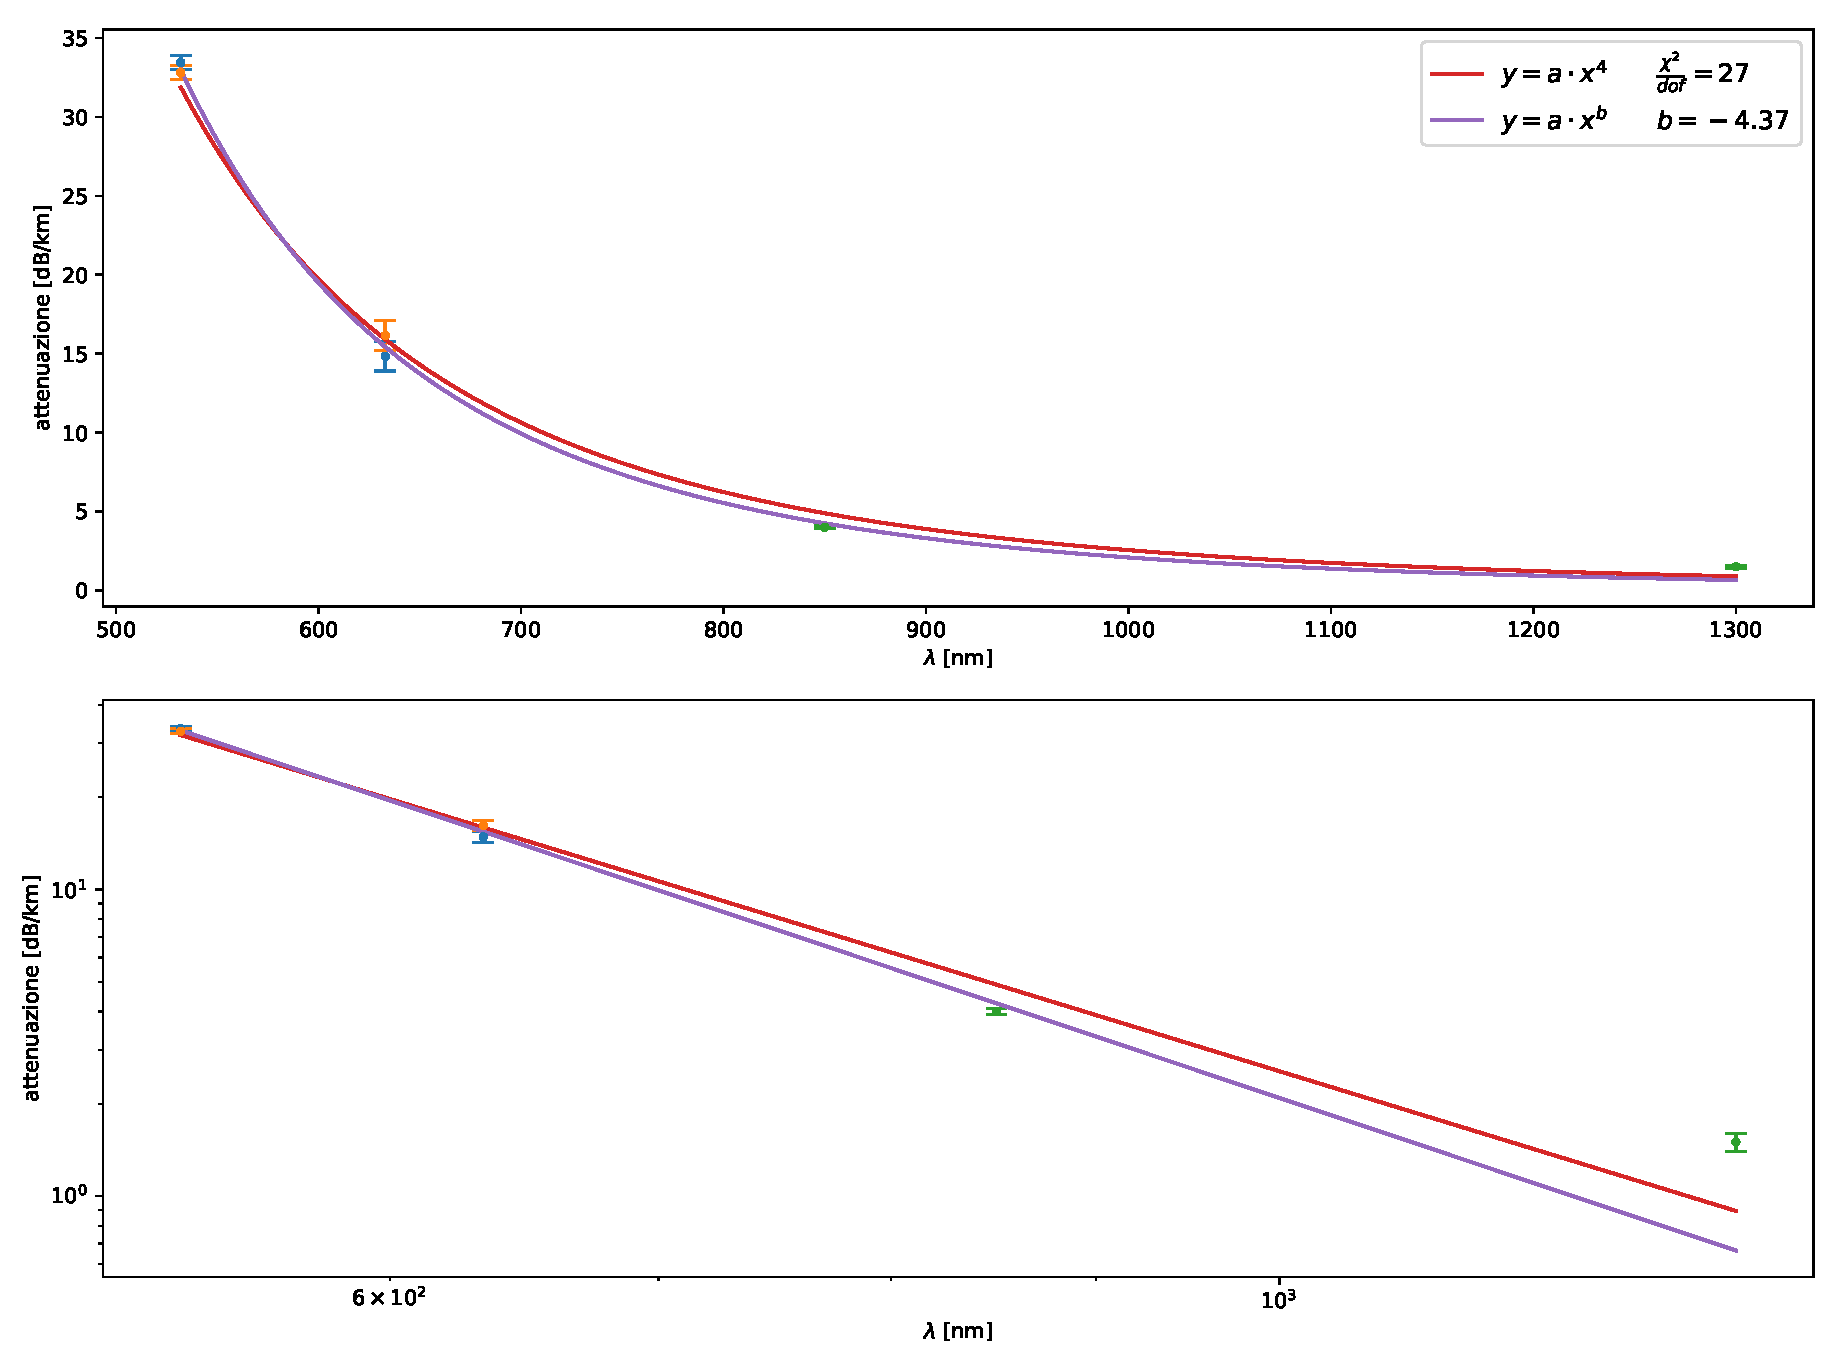
\includegraphics[width=\textwidth]{attenuazione_tutti.pdf}
	\caption{Grafico dell'attenuazione in fibra ottica sia in scala lineare che bilogaritmica. In blu e arancione le nostre misure, in verde i valori del datasheet.}
	\label{fig:attenuazione_tutti}
\end{figure}



\section{Propagazione modo LP$_{01}$ in una fibra SM}

\subsection{Teoria}

\subsection{Presa dati}

1 tabella

\subsection{Analisi dati}

1 plot

\section{Propagazione modi superiori}

\subsection{Teoria}

\subsection{Presa dati}

\subsection{Analisi dati}

\section{Fibra a conservazione di polarizzazione}

\subsection{Teoria}

\subsection{Presa dati}

\subsection{Analisi dati}

1 figura

\section{Lente GRIN}

\begin{multicols}{2}


\subsection{Teoria}
Una lente GRIN (da GRadient-INdex) � un cilindro fatto di materiale rifrangente con indice di rifrazione variabile a seconda della distanza dall'asse.
\begin{figure}[H]
	\centering
	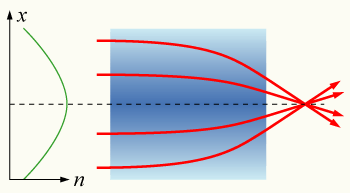
\includegraphics[width=0.4\textwidth]{Grin-lens.png}
\end{figure}
Una lente GRIN tagliata a $\lambda/4$ focalizza assi parassiali sulla superficie e viceversa. La lente GRIN a nostra disposizione � tagliata a 0.29$\lambda$ quindi focalizza onde sferiche ad una certa distanza dalla superficie.

\subsection{Coefficiente di accoppiamento}
L'idea � usare la lente GRIN per lanciare luce in fibra. Misuriamo quindi il coefficiente di accoppiamento di una sorgente laser o LED a una fibra ottica multimodo attraverso una lente GRIN.
Il coefficiente di accoppiamento si ottiene con la formula
\[\Gamma = 10 \log\left |\frac{P_{in}}{P_{out}} \right|\]
\subsubsection*{Procedura e accorgimenti}
$P_{in}$ � la potenza in ingresso, misurata con il \textit{power meter} a diretto contatto con la sorgente, e $P_{out}$ � la potenza in uscita, misurata, con lo stesso \textit{power meter}, all'uscita della fibra ottica.

$P_{out}$ dipende dall'allineamento l'apparato, la sua misura non � quindi ripetibile a meno di non ottenere lo stesso identico allineamento. Pertanto abbiamo scelto, per convenzione, di variare l'allineamento fino a registrare il massimo valore di $P_{out}$, in questo modo altri studenti che utilizzino il nostro apparato e seguano la stessa procedura devono trovare il medesimo valore. Allo stesso modo $P_{in}$ � la massima potenza registrata con la sorgente a diretto contatto con il sensore.

La corrente di alimentazione varia lentamente in funzione del tempo (effetti $1/f$) quindi ci siamo assicurati che le misure di $P_{in}$ e $P_{out}$ avvenissero con la stessa alimentazione. La misura che richiede pi� pazienza � quella di $P_{out}$, quindi l'abbiamo misurata per prima e immediatamente dopo abbiamo misurato $P_{in}$, verificando che l'alimentatore fornisse la stessa corrente.

\subsubsection*{Risultati}
\begin{table}[H]
	\centering
	\begin{tabular}{|c|cccc|}
		\hline
		& $I_{in}$ [mA]  & $P_{out}$ [mW]& $P_{in}$ [mW]& $\Gamma [dB]$ \\
		\hline
		laser  & 78.0(1) & 3.50(1) & 6.19(6) & 2.48(4)\\

		LED & 81.1(2) & 0.00491(2) & 8.21(10) & 32.23(6)\\
		\hline
	\end{tabular}
	\caption{Coefficiente di accoppiamento. L'errore sulla corrente � la digitalizzazione, gli errori sulle potenze una nostra stima in base alle fluttuazioni delle misure.}
	\label{tab:GRIN}
\end{table}

In Tabella \ref{tab:GRIN} ci sono i dati raccolti ed il coefficiente di accoppiamento ricavato:
\begin{align*}
	\Gamma_{laser} &= 2.48(4) \textrm{ dB}\\
	\Gamma_{LED} &= 32.23(6) \textrm{ dB}
\end{align*}

\subsection{Trasmissione di un segnale}
Modulando l'intensit� della luce lanciata in fibra � possibile trasmettere un segnale.
\begin{figure}[H]
	\centering
	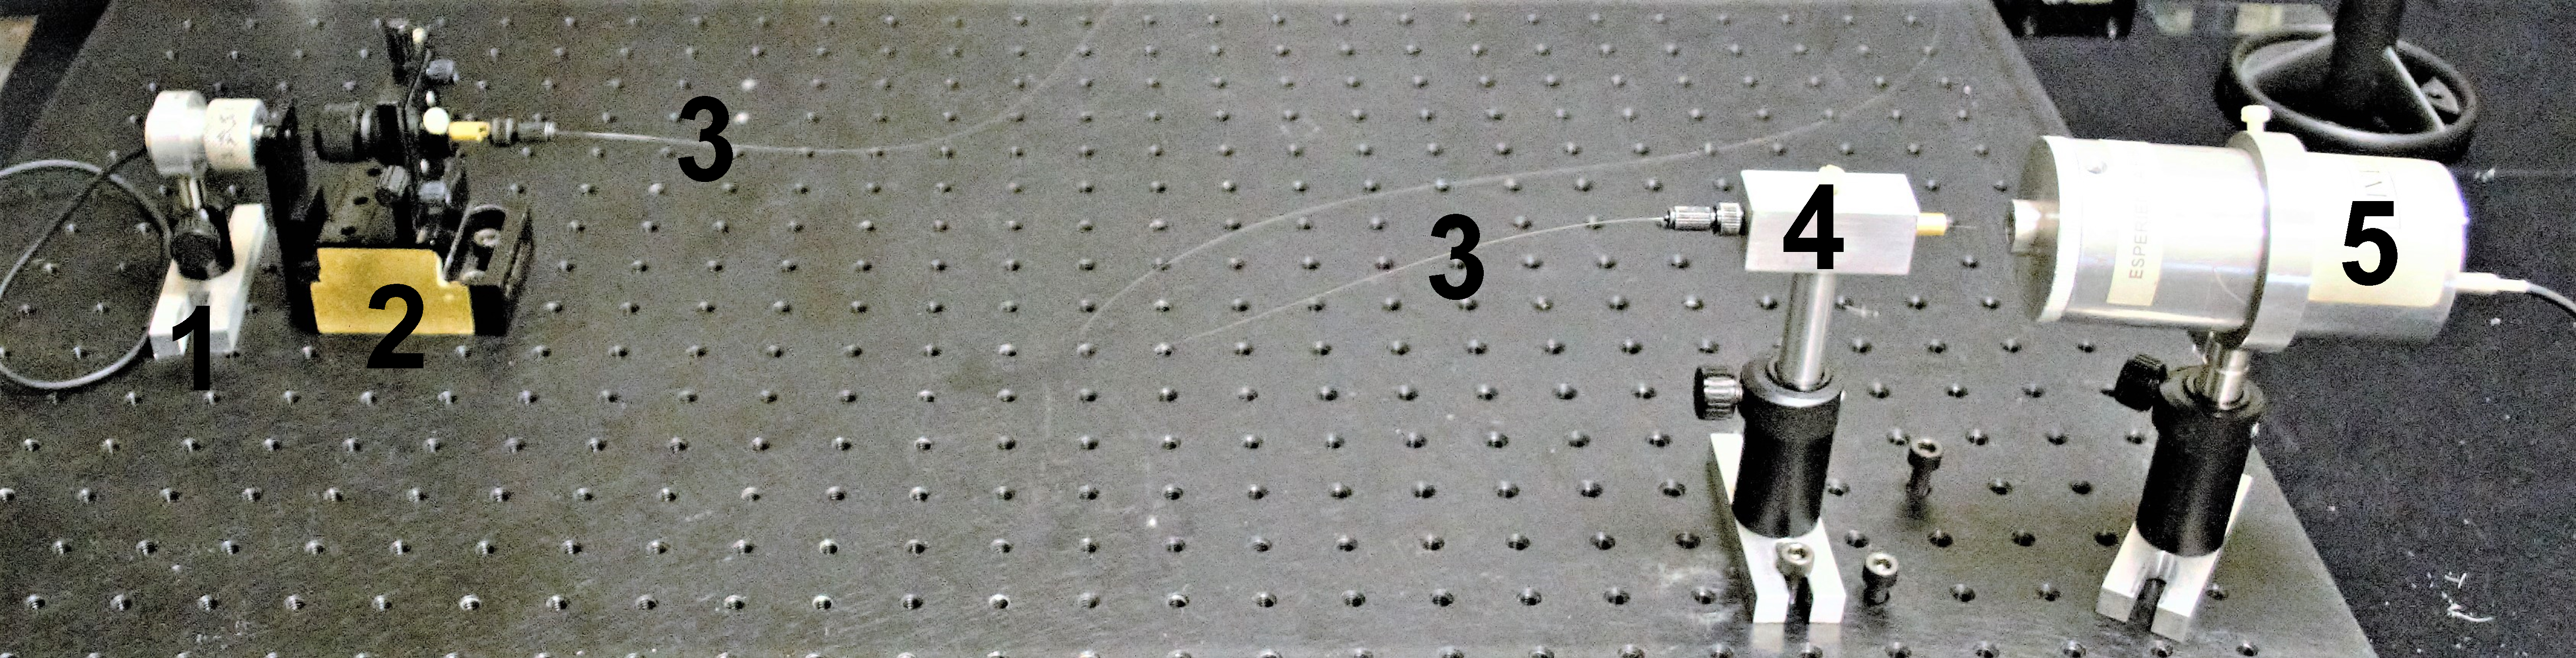
\includegraphics[width=0.5\textwidth]{apparato_segnale_acustico.pdf}
	\caption{Apparato sperimentale per la trasmissone di un segnale.}
	\begin{enumerate}
		\item Diodo laser
		\item Lanciatore (con lente GRIN)
		\item Fibra ottica
		\item Uscita della fibra
		\item Rilevatore al silicio
	\end{enumerate}
	\label{fig:apparato_segnale}
\end{figure}

In Figura \ref{fig:apparato_segnale} � rappresentato l'apparato sperimentale che utilizziamo. Il diodo laser � alimentato da una corrente modulata con un piccolo segnale prodotto da un generatore di funzioni.\\
Il rilevatore, che trasforma il segnale ottico in una tensione, � collegato ad un amplificatore che trasforma la tensione in segnale acustico, che sentiamo ad orecchio.

Registriamo il segnale acustico grazie ad un'app gratuita per cellulare per accordare gli strumenti musicali.
In Figura \ref{fig:segnale_acustico} sono riportati gli screenshot delle 3 misure effettuate:
\begin{enumerate}
	\item Segnale dato dalla luce ambientale. La stanza � illuminata da lampade al neon, che viene eccitato al doppio della frequenza della corrente alternata, quindi circa a 100-120 Hz. Misuriamo 98 Hz.
	\item Segnale del generatore di funzioni: regoliamo la frequenza fino ad intonare un la5 (880 Hz).
	\item Segnale del generatore di funzioni: regoliamo la frequenza fino ad intonare un la4 (440 Hz).
\end{enumerate}

\begin{figure}[H]
	\centering
	\begin{minipage}{0.148\textwidth}
		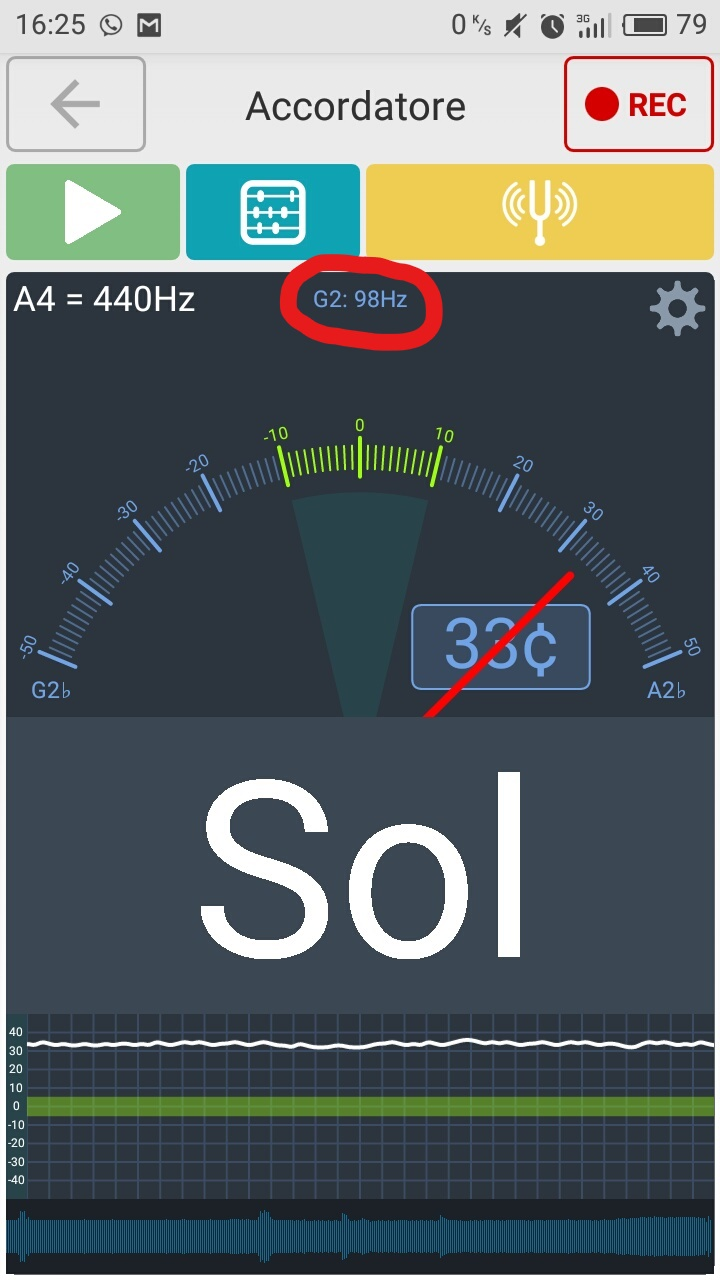
\includegraphics[width=\textwidth]{sol2.png}
	\end{minipage}
	\begin{minipage}{0.16\textwidth}
		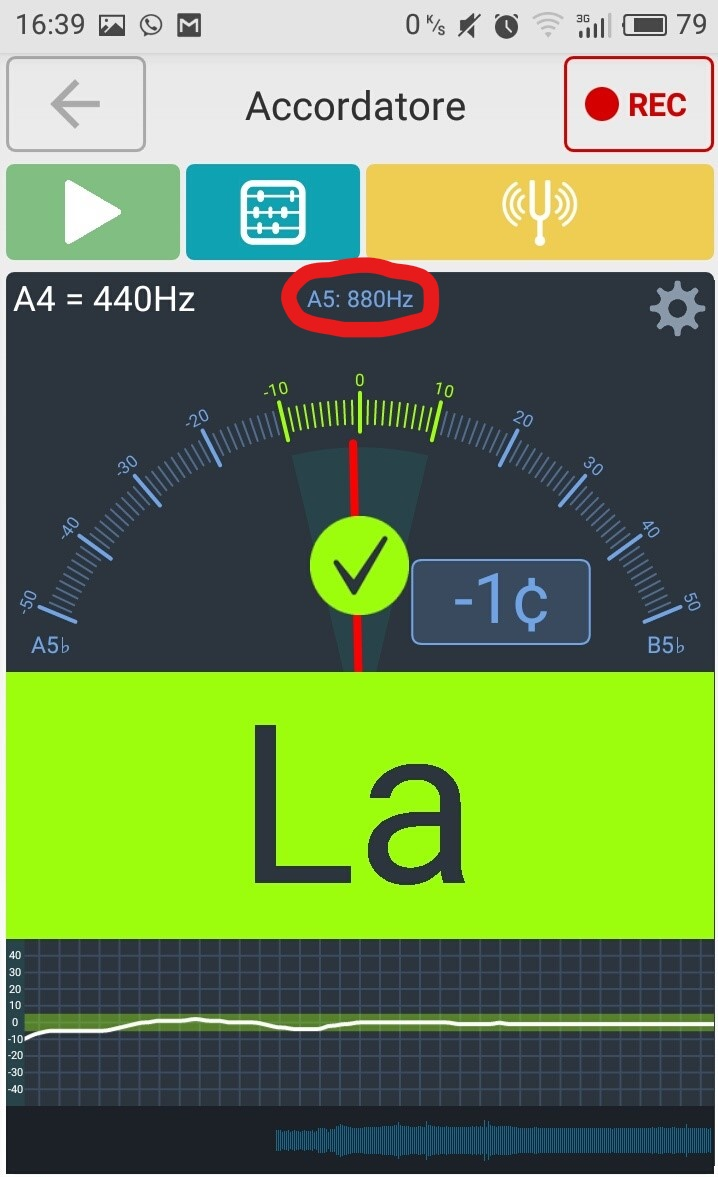
\includegraphics[width=\textwidth]{la5.png}
	\end{minipage}
	\begin{minipage}{0.16\textwidth}
		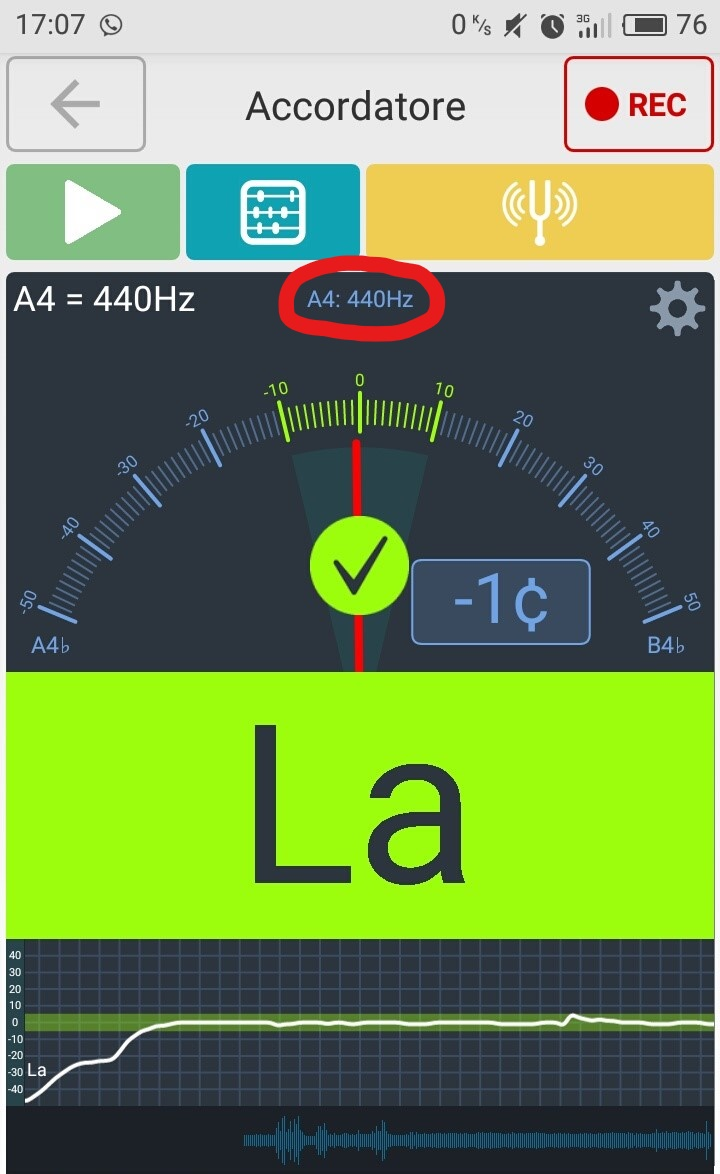
\includegraphics[width=\textwidth]{la4.png}
	\end{minipage}
	\caption{Screenshot del cellulare che misura la frequenza, cerchiata in rosso.}
	\label{fig:segnale_acustico}
\end{figure}

\end{multicols}
	
\end{document}